\documentclass{article}

% if you need to pass options to natbib, use, e.g.:
% \PassOptionsToPackage{numbers, compress}{natbib}
% before loading nips_2017
%
% to avoid loading the natbib package, add option nonatbib:
% \usepackage[nonatbib]{nips_2017}

\usepackage[final]{nips_2017}

\usepackage{multicol}
\usepackage{graphicx}
\usepackage[utf8]{inputenc} % allow utf-8 input
\usepackage[T1]{fontenc}    % use 8-bit T1 fonts
\usepackage{hyperref}       % hyperlinks
\usepackage{url}            % simple URL typesetting
\usepackage{booktabs}       % professional-quality tables
\usepackage{amsfonts}       % blackboard math symbols
\usepackage{nicefrac}       % compact symbols for 1/2, etc.
\usepackage{microtype}      % microtypography

\usepackage{amsmath}
\usepackage{caption}

\def\apeqA{\SavedStyle\sim}
\def\apeq{\setstackgap{L}{\dimexpr.5pt+1.5\LMpt}\ensurestackMath{%
      \ThisStyle{\mathrel{\Centerstack{{\apeqA} {\apeqA} {\apeqA}}}}}}
\newcommand{\lstm}{LSTM }

% Choose a title for your submission
\title{Project 2: Predicting the End of a Story}

\author{Student 1 \qquad Student 2 \qquad Student 3}

\begin{document}
% \nipsfinalcopy is no longer used

\maketitle

% We do not requrire you to write an abstract. Still, if you feel like it, please do so.
%\begin{abstract}
%\end{abstract}

%Feel free to add more sections but those listed here are strongly recommended.

\section{Introduction}
\label{sec:intro}

In the recent years, the NLP community has been trying to fully implement deep
language understanding by representing and learning commonsense knowledge.
However, understanding casual and correlational relationships between events is
still extremely challenging. Recently, a new framework for assesing story
understanding ans script learning has been published: the {\it 'Story Cloze
    Test'} to provide research an evaluation framework for understanding casual
and correlational relationships between events. In this report, we describe
several approaches explored for solving the 'Story Cloze Test'. Our approaches
range from analyzing sentiment trajectory of stories to neural network models
inspired in previous research. We report the accuracy for both the validation
and test sets.

%Natural language is
%You can keep this short. Ideally you introduce the task already in a way that highlights the difficulties  your method will tackle.

\section{Methodology}
\label{sec:general}

The idea of our approach follows that of successes in previous work such as
\cite{UWNLP}, \cite{Goel} and \cite{COGCOMP}. More specifically, our approach
consists of training a binary classifier based on an augmented data set which we
create ourselves. This data augmentation is based on previously successful ideas
applied to this task \cite{LSTMClassifier, SENTENCE_EMB}.  The features for our
classifier are generated by a set of feature extractors which produce a vector
of features for any 5 sentence story. Each feature extractor is a different
model that is first fit and then used for extracting such features.

We now explain the different stages required for training our model.

\textbf{Data augmentation.} The augmented data set is composed of 5 labeled
sentence stories. We create this data set by combining the original ROCStory
corpus, introduced in \cite{ROCstories}, and a negative data set. Here the ROC
dataset gets assigned a positive label and the negative set a negative label. We
compose the negative dataset by replacing the ending of each 5 sentence story by
a randomly selected ending, as done by \cite{LSTMClassifier} and
\cite{SENTENCE_EMB}. Throughout this paper we use a replication factor of 1,
i.e., for every sample of the original training set, we add a single negative
sample.

\textbf{Feature extraction.} To obtain the features for our logistic regression
model, we use what we named {\it feature extractors}. A feature extractor is
simply a model which takes in a 5 sentence story and outputs a feature or vector
of features. Feature extractors are described in depth in section
\ref{sec:extractors}. Then, to obtain the final set of features we simply
combine the features obtained for each sample from each extractor.

\textbf{Classification.} After extracting features, we fit our classifier to be
able to distinguish between a fake (negative) story and a real (positive) one.
We opted for using a binary logistic regression as it has been already explored
successfully in previous works \cite{UWNLP,Goel,COGCOMP}.

%Your idea. You can rename this section if you like. Early on in this section -- but not necessarily first -- make clear what category your method falls into: Is it generative? Discriminative? Is there a particular additional data source you want to use?

\section{Model}

	\begin{figure}[h!]
		\centering
		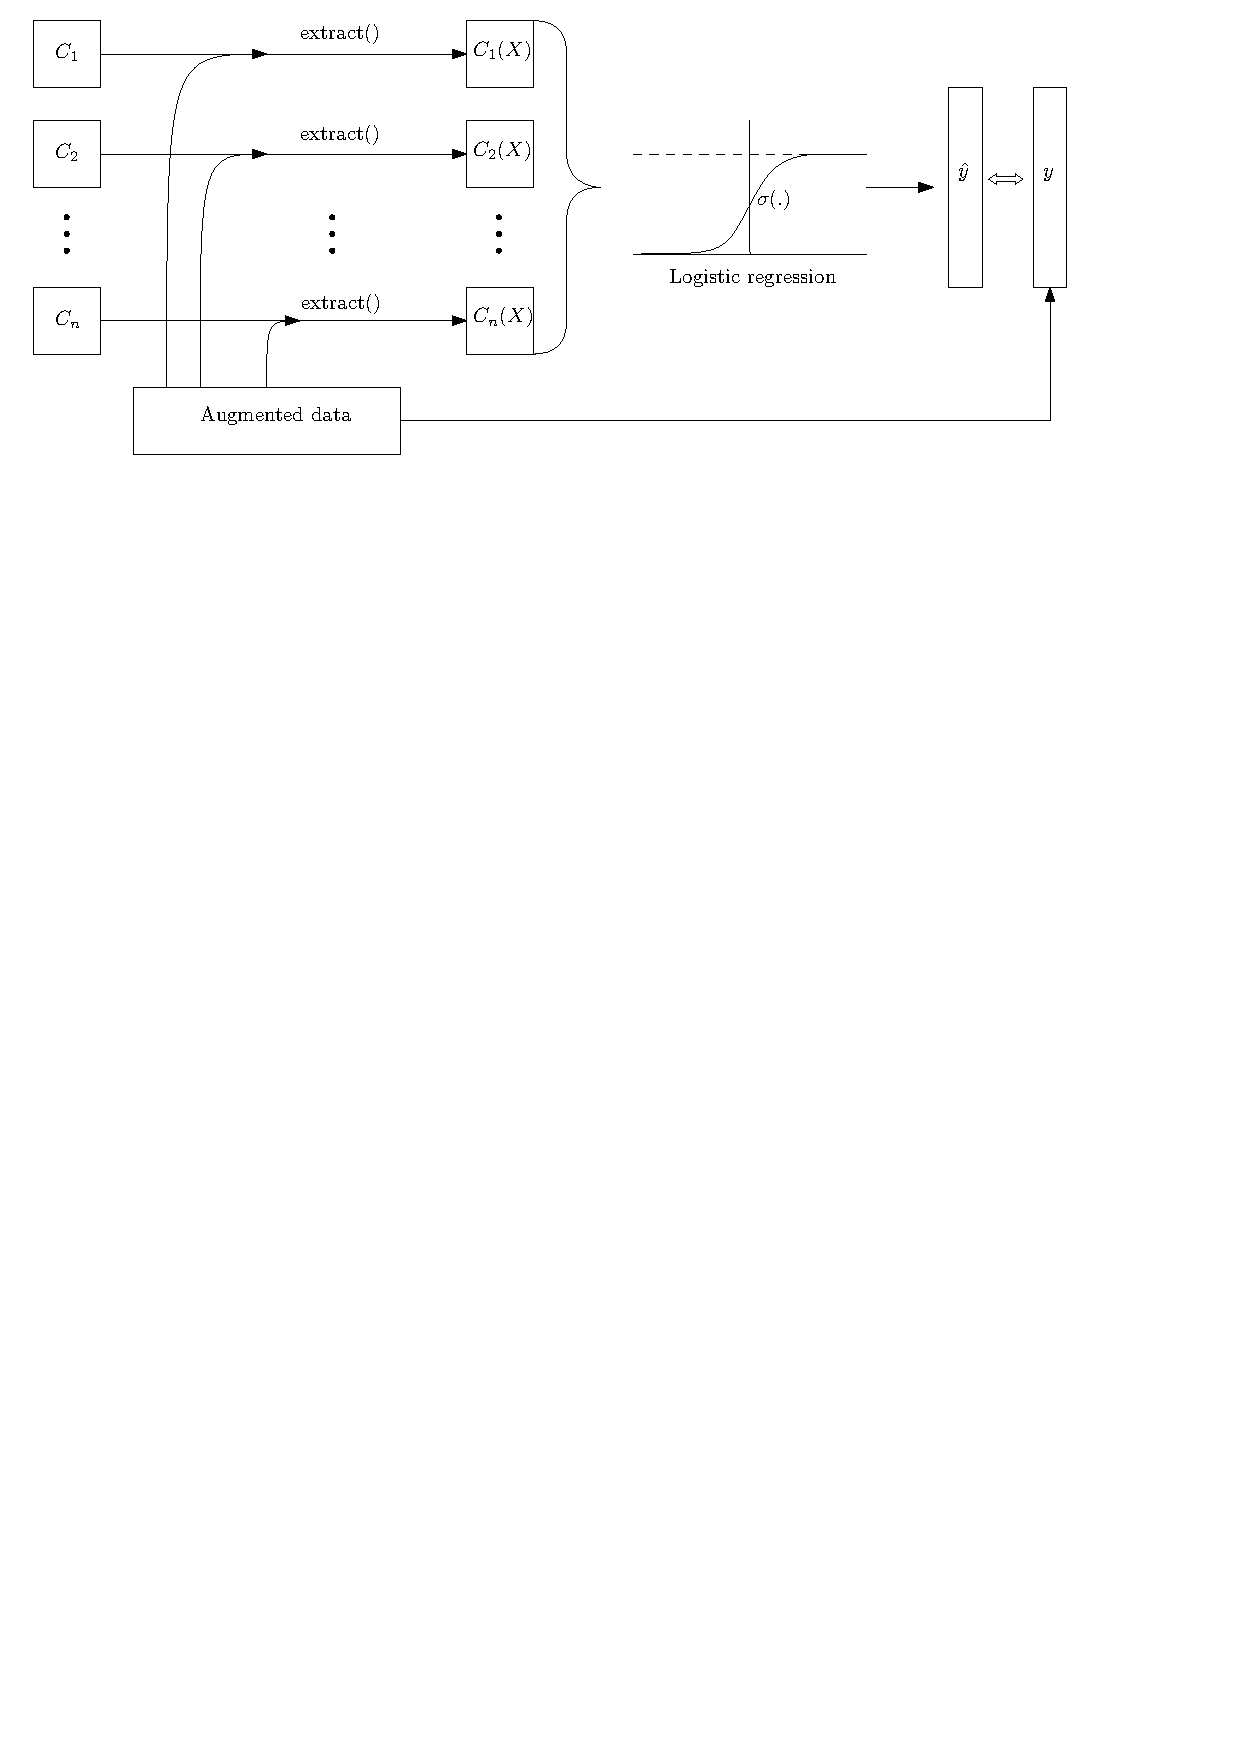
\includegraphics[scale=0.6]{fig/logistic_fitting.pdf}
		\caption{Main components of the global approach.}
		\label{Main}
	\end{figure}

The core components of our approach can be seen in figure \ref*{Main}. As
previously described, each $C_i$ is a feature extractor and indicates a mapping:
%
\begin{equation} C_i: \mathbb{S}^5 \rightarrow \mathbb{R}^{l(i)} \end{equation}
%
That is a mapping function of the set of all 5 sentence stories ($\mathbb{S}^5$)
to a real vector. Note that not all extractors need to map to the same length
vectors and that all the feature extractions use the augmented dataset. This is
denoted by $C_i(X)$ in figure \ref*{Main}. Then, we apply logistic regression
using the Scikit-learn implementation \cite{SKL} to the extracted set of
features and the labels of the augmented set.

\subsection{Fitting extractors}

In order to extract features from 5 sentence stories, the extractors have to be
fitted first. For extractors which training takes longer, we load the
pre-trained model to be used. Moreover, each extractor receives either an
augmented data set or the original ROC data set.

%\begin{figure}[h!]
%	\centering
%	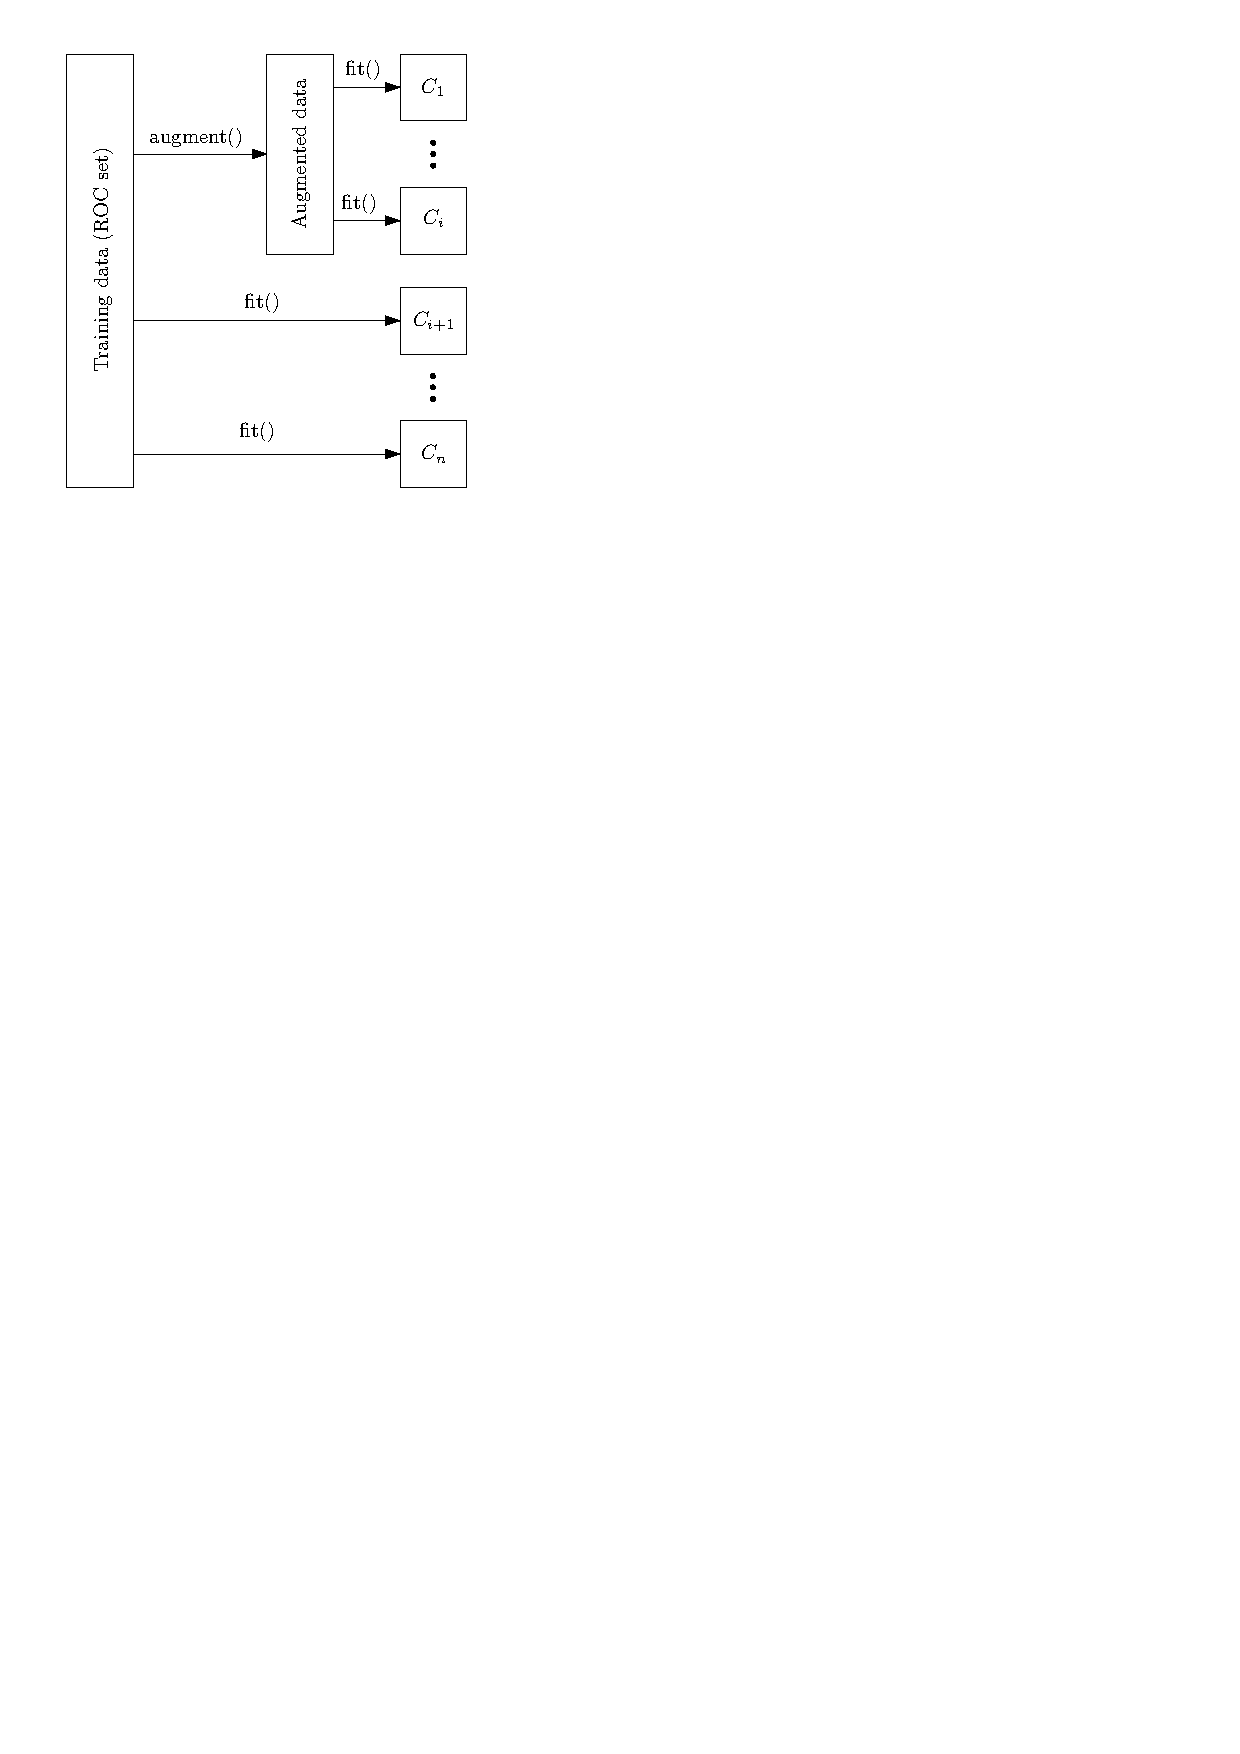
\includegraphics[scale=0.8]{fig/extractors_fitting.pdf}
%	\caption{Fitting feature extractors by using the Original ROC set or the augmented set.}
%	\label{fit}
%\end{figure}

\subsection{Different extractors}
\label{sec:extractors}

Next, we discuss various feature extraction methods we implemented in the model
in extensive detail.

\textbf{Sentiment trajectory} This feature was previously explored by \cite{COGCOMP} and is based in the fact that stories often follow a certain emotional path. e.g. a story with a positive introduction might have a sad climax but a happy ending. In this feature we consider a story to be built in blocks as follows: the first sentence forms the introduction ($1$), the second and third form the body ($2$), the fourth forms the climax ($3$) and fifth forms the ending ($4$)\footnote{We have explored multiple ways of categorising the sentences in blocks and found this configuration to be the most effective, which is in allignment with \cite{COGCOMP}.}.To model the sentiment of the trajectory from (1) to (4) let the following be a joint distribution:

\begin{equation}
\label{eq:categorical}
(S_1, S_2,S_3,S_4) \sim Cat(\{-1,0,1\}^4, \theta)
\end{equation}
Where $S_i$ is the sentiment of the $i$'th block as defined above. We consider the possible outcomes of $S_i$ to be in the set $\{-1,0,1\}$ denoting a negative, neutral and positive sentiment respectively.  As seen in (\ref{eq:categorical}) we model the joint distribution of the sentiment trajectory as categorical over the set of all possible trajectories of length 4. To estimate the parameters $\theta$ in this model, we considered the maximum a-posteriori estimate (MAP) with a Dirichlet (conjugate) prior. That is we denote $\theta_{s_1,s_2,s_3,s_4} = P(S_1 = s_1, S_2=s_2, S_3=s_3, S_4=s_4)$ and given a set of $N$ 5 sentence stories we estimate it as follows:
\begin{equation}
\label{eq:estimate_sentiment}
\begin{split}
\hat{\theta}_{s_1,s_2,s_3,s_4} &= \frac{count(s_1,s_2,s_3,s_4) + \alpha - 1}{\sum\limits_{s_1,s_2,s_3,s_4}(count(s_1,s_2,s_3,s_4) + \alpha-1) }\\
&=\frac{count(s_1,s_2,s_3,s_4) + \alpha - 1}{N + 81(\alpha-1) }
\end{split}
\end{equation}
Here $\alpha$ is the concentration parameter of the dirichlet prior. In our implementation we choose $\alpha_1 = ... = \alpha_{81} = \alpha$.
\begin{itemize}
	\item \textit{Fitting}: fitting this extractor consists of estimating the parameters as in (\ref{eq:estimate_sentiment}) given the original \textbf{non augmented} dataset.
	\item \textit{Extracting}: extracting features from a 5 sentence story consists then of finding how likely the trajectory is, i.e. the feature is $P(S_1 = s_1, S_2=s_2, S_3=s_3, S_4=s_4)$ using the estimated parameters.
	\item \textit{Implementation}: In our implementation we used the Natural Language Tool Kit's (NLTK \cite{NLTK_VADER}) implementation of VADER sentiment analasys \cite{VADER} to analyse the sentiment of the different story blocks.
\end{itemize}

\textbf{Embedded closeness} Based on the idea that the ending of a story should stay consistent with the everything that came before it. e.g. the ending of a story about a chef will probably have more connectin to food than to fashion. We take a similar approach to previously considered approaches AveMax of \cite{LSTMClassifier} and Topic Consistency of \cite{COGCOMP}.
This feature consists of a three-step process i.e. given a 5 sentence story we do the following:
\begin{enumerate}
	\item A POS tagger is used on the entire story and following \cite{COGCOMP} we only consider the topic words. We chose nouns, verbs and adjectives to form the topic words.\footnote{The full set of POS tags we consider is: JJ, JJR, JJS for adjectives; NN, NNS, NNP, NNPS for  nouns and VBD, VBG, VBN, VBP, VBZ for verbs. The tags are defined in \cite{TREEBANK}}
	\item We use pre-trained word embeddings of dimension 50 and replace each of the topic words with its respective embedding.
	\item For each topic word in the last sentence the cosine similarity is measured to each topic word in the previous four sentences, using the embeddings. We then only consider the maximum similarity measured for each topic word in the last sentence. Lastly we take the average of the maximum measured similarities. 
\end{enumerate}
This procedure results in a single value we denote as the \textit{embedded closeness} of a story and measures the level of consistency of a ending to the previous four sentences.
\begin{itemize}
	\item \textit{Fitting}: there is no fitting in this model.
	\item \textit{Extracting}: given a 5 sentence story we apply previously described procedure to obtain an embedded closeness score. The feature is this embedded closeness.
	\item \textit{Implementation}: We use NLTK's POS tagger to find topic words \cite{NLTK_VADER}. We use Stanfords pre-trained GloVe word embeddings \cite{GLOVE} trained on 6 billion tokens, vocabulary size 400000  and of dimension 50.
\end{itemize}
%The math/architecture of your model. This should formally describe your idea from above. If you really want to, you can merge the two sections.

\textbf{Language Model} Intuitively to humans some sentences make more sense than others. e.g. \textit{Jack moved recently! He picked up his home and placed it somewhere else} would make little to no sense for most humans. The key idea of this feature is to extend this to the level of stories. In order to exploit this, we took a similar approach to \cite{UWNLP} and trained an LSTM language model to define a probability distribution over a vocabulary of words given a context. 
\begin{itemize}
	\item \textit{Fitting:} when fitting the language model we use the original training set.
	\item \textit{extracting}: given a 5 sentence story we use the trained model to find the probability of the entire story i.e. we find:
	\begin{multicols}{2}
		\begin{equation}
		P(w_1, ..., w_n) = \prod_{i=1}^{n} P(w_i|h_i)
		\end{equation}\break
		\begin{equation}
		p(w_i|h_i) = \frac{exp(W_ih_i)}{\sum_{j=1}^{V}exp(W_jh_i)}
		\end{equation}
	\end{multicols}
	where $w_1, ..., w_n$ are all the words in the story, $h_i$ is the output of the LSTM cell at timestep $i$, $V$ is the vocabulary size and $W_i$ is a row of the weight matrix $W$ which corresponds with a dense layer. The feature is this probability.
	\item \textit{implementation}: To implement the LSTM language model we used keras \cite{KERAS}. We used Stanfords pre-trained GloVe word embeddings trained on 6 billion tokens, vocabulary size $400000$ and of dimension 50. We used a singe LSTM layer with hidden size of 100, the vocabulary was limited to $10 000$ tokens. Optimization was done using the built in Adam optimizer.
	
\end{itemize}

\textbf{LSTM classifier} Similarly 

\section{Training}
\label{sec:training}
%What is your objective? How do you optimize it?

In this section, we describe the results for the different extractors we apply
to the {\it Story Cloze task} as well as for our Ensemble method. For all our
approaches, the training set is first augmented as previously explained and then
used to train each of our extractors.

Table \ref{tab:params} shows the number of trainable parameters of the models we
used for the task and additionally the training duration. Our models were
trained using 15\% of the entire training data as validation data for training.
The accuracy with the actual validation set is evaluated after training is
completed. 

\begin{table}[h!]
    \caption{Feature extractors.}
    \begin{center}
        \label{tab:params}
        \begin{tabular}{||c c c c c||} 
            \hline
            Method                 & \# Trainable parameters   & Training               & \# Validation set         & Test set \\ [0.5ex] 
            \hline\hline
            Sentiment trajectory   & 80                        & $ \approx $ 45 secs.   & \textbf{61.2\%}           & \textbf{60.4\%} \\ 
            \hline
            Embedded closeness     & 0                         & $ \approx $ 5 secs.    & 56.5\%                    & 55.4\% \\
            \hline
            LSTM classifier        & $ \approx $ 200K          & 20 epochs              & 54.03\%                   & 51.3\% \\ 
            \hline
            Language model         & $ \approx $ 1M            & 20 epochs              & 51.2\%                    & 50.02\% \\
            \hline
            \textbf{Ensemble}      & 80                        & $ \approx $ 45 secs.   & \textbf{61.2\%}           & \textbf{60.4\%} \\ [1ex] 
            \hline
        \end{tabular}
    \end{center}
\end{table}

The \lstm classifier was trained for 20 epochs using 15\% of the entire training
data as validation data for training. We did not perform more training epochs
due to the fact that we observed a decrease in the validation accuracy and an
increase of the loss function, i.e., the model was overfitting.  The language
model was trained for 20 epochs using a similar configuration as the \lstm
classifier. We observed that the loss function was still improving with the
number of epochs done. The sentiment trajectory method is based on using a
random forest classifier, thus its training phase is similar to other
classification methods and in this case is not time consuming.

\section{Results}
\label{sec:results}

Table \ref{tab:params} also shows the accuracy obtained by different methods on the
validation and the provided test set. 


%\begin{table}
%    \caption{Accuracy on different data sets.}
%    \begin{center}
%        \label{tab:results}
%        \begin{tabular}{||c c c||} 
%            \hline
%            Method                 & \# Validation set         & Test set \\ [0.5ex] 
%            \hline\hline
%            Sentiment trajectory   & 61.2\%                    & \textbf{60.4\%} \\ 
%            \hline
%            Embedded closeness     & 56.5\%                    & 55.4\% \\
%            \hline
%            LSTM classifier        & 54.03\%                   & 51.3\% \\ 
%            \hline
%            Language model         & 51.2\%                    & 50.02\% \\ [1ex] 
%            \hline
%        \end{tabular}
%    \end{center}
%\end{table}

Our approaches based on neural models were not able to perform as expected on
this task. For example, the \lstm classifier scored really high while training
(around 80\% accuracy). However it was not table to perform so well for the
task. This is because the model is able to capture sentences with the same
content, i.e., sentences containing the same subject, similar verbs and so on,
but not all stories contain the same subjects and verbs. Many times the stories
have a twist that our model is not able to capture although it might be obvious
for a human. Moreover, our language model was not able to go beyond a 50\%
accuracy on the test set. 

On the other hand, the sentiment trajectory model is able to capture the how the
story is actually evolving along the sentences. Thus, with this method we were
able to score a high accuracy on both data sets.

%This {\bf must} at least include the accuracy of your method on the validation set.

\section{Conclusion}
You can keep this short, too. \cite{*}

\bibliographystyle{plain}
\bibliography{bib/refs}
\end{document}
